%%%%%%%%%%%%%%%%%%%%%%%%%%%%%%%%%%%%%%%%%
% a0poster Landscape Poster
% LaTeX Template
% Version 1.0 (22/06/13)
%
% The a0poster class was created by:
% Gerlinde Kettl and Matthias Weiser (tex@kettl.de)
% 
% This template has been downloaded from:
% http://www.LaTeXTemplates.com
%
% License:
% CC BY-NC-SA 3.0 (http://creativecommons.org/licenses/by-nc-sa/3.0/)
%
%%%%%%%%%%%%%%%%%%%%%%%%%%%%%%%%%%%%%%%%%

%----------------------------------------------------------------------------------------
%	PACKAGES AND OTHER DOCUMENT CONFIGURATIONS
%----------------------------------------------------------------------------------------

\documentclass[a0,landscape]{a0poster}

\usepackage{multicol} % This is so we can have multiple columns of text side-by-side
\columnsep=100pt % This is the amount of white space between the columns in the poster
\columnseprule=3pt % This is the thickness of the black line between the columns in the poster

\usepackage[svgnames]{xcolor} % Specify colors by their 'svgnames', for a full list of all colors available see here: http://www.latextemplates.com/svgnames-colors

\usepackage{times} % Use the times font
%\usepackage{palatino} % Uncomment to use the Palatino font

\usepackage{graphicx} % Required for including images
\graphicspath{{figures/}} % Location of the graphics files
\usepackage{booktabs} % Top and bottom rules for table
\usepackage[font=small,labelfont=bf]{caption} % Required for specifying captions to tables and figures
\usepackage{amsfonts, amsmath, amsthm, amssymb} % For math fonts, symbols and environments
\usepackage{wrapfig} % Allows wrapping text around tables and figures

\usepackage{natbib}

\begin{document}

%----------------------------------------------------------------------------------------
%	POSTER HEADER 
%----------------------------------------------------------------------------------------

% The header is divided into three boxes:
% The first is 55% wide and houses the title, subtitle, names and university/organization
% The second is 25% wide and houses contact information
% The third is 19% wide and houses a logo for your university/organization or a photo of you
% The widths of these boxes can be easily edited to accommodate your content as you see fit

\begin{minipage}[b]{0.75\linewidth}
\veryHuge \color{NavyBlue} \textbf{Pleiotropy vs. Close Linkage in the Diversity Outbred Mouse Population} \color{Black}\\ % Title
%\Huge\textit{An Exploration of Complexity}\\[1cm] % Subtitle
\huge \textbf{Fred Boehm$^{\dagger}$, Mark Keller$^{\dagger}$, Alan Attie$^{\dagger}$, Mary Rabaglia$^{\dagger}$, Kathy Schueler$^{\dagger}$, Donald Stapleton$^{\dagger}$, Gary Churchill$^{\ddagger}$, Brian Yandell$^{\dagger}$, and Karl Broman$^{\dagger}$}\\ % Author(s)
\huge University of Wisconsin-Madison$^{\dagger}$ \& The Jackson Laboratory$^{\ddagger}$\\ % University/organization
\end{minipage}
%
\hspace{8cm}
\begin{minipage}[b]{0.2\linewidth}
\color{DarkSlateGray}\Large \textbf{Contact Information:}\\
Department of Statistics\\ % Address
University of Wisconsin-Madison\\
%1220 Medical Sciences Center, 1300 University AVE\\
Email: \texttt{fred.boehm@wisc.edu}\\ % Email
Website: \texttt{http://fboehm.github.io/}
\end{minipage}
%
%\begin{minipage}[b]{0.19\linewidth}
%
\includegraphics[width=10cm]{logo.png} % Logo or a photo of you, adjust its dimensions here
%\end{minipage}

\vspace{1cm} % A bit of extra whitespace between the header and poster content

%----------------------------------------------------------------------------------------

\begin{multicols}{4} % This is how many columns your poster will be broken into, a poster with many figures may benefit from less columns whereas a text-heavy poster benefits from more

%----------------------------------------------------------------------------------------
%	ABSTRACT
%----------------------------------------------------------------------------------------

\color{Navy} % Navy color for the abstract

%\begin{abstract}

%We present initial results from our studies to differentiate pleiotropic QTl from closely linked QTL. In the context of univariate QTL mapping studies, we found numerous loci that associated with multiple clinical traits. To better understand the nature of these associations, we sought to distinguish pleiotropic effects, in which a single locus associates with multiple traits, from closely linked, but distinct, loci, in which two nearby genetic loci each associate with a single trait. We present a likelihood ratio test to quantitatively assess pleiotropy vs. close linkage for two traits that map to a small genomic region. 

%\end{abstract}

%----------------------------------------------------------------------------------------
%	INTRODUCTION
%----------------------------------------------------------------------------------------

\color{SaddleBrown} % SaddleBrown color for the introduction
\section*{Introduction}

Methods for distinguishing a single pleiotropic genomic locus from multiple, closely linked loci have significant implications in modern genetics research. Such strategies may reveal novel roles for known genes and may contribute to discovery of previously unstudied genes. In both cases, our methods enhance understanding of the genetic underpinnings of complex traits. 




%----------------------------------------------------------------------------------------
%	OBJECTIVES
%----------------------------------------------------------------------------------------

\color{DarkSlateGray} % DarkSlateGray color for the rest of the content

\section*{Goal}

\begin{itemize}
\item Are two traits affected by a single locus (pleiotropy) or a pair of loci (close linkage)? 
\end{itemize}

%----------------------------------------------------------------------------------------
%	MATERIALS AND METHODS
%----------------------------------------------------------------------------------------

\section*{Methods}

\subsection*{Likelihood ratio test development}

\begin{itemize}
\item \cite{jiang1995multiple} developed a likelihood ratio test to characterize two jointly mapped traits as either both being associated with a single pleiotropic locus or each being associated with distinct (but closely linked) loci
\item Extend the methods of \cite{jiang1995multiple} to accommodate the eight founder haplotypes in the Diversity Outbred (DO) mouse population
\item Implement a likelihood ratio test for the competing hypotheses:

\begin{eqnarray}
H_0: & \lambda_1 = \lambda_2\nonumber \\
H_a: & \lambda_1 \neq \lambda_2\nonumber
\end{eqnarray}
\begin{itemize}
\item $\lambda_1$ is the genomic location for the first QTL, while $\lambda_2$ is the genomic location for the second QTL
\item $H_0$ is equivalent to pleiotropy, while $H_a$ is close linkage
\end{itemize}
\item Initially limit our analysis to two traits
\item We modeled the two phenotypes, together, as arising from normal distributions that depend on the estimated founder haplotype probabilities.
\begin{equation}
Y = XB + E
\end{equation}
\begin{itemize}
\item $Y$ is a n x 2 matrix of phenotype values, $X$ is the n x 8 matrix that includes a column of ones and 7 of the 8 estimated haplotype probabilities, $B$ is the 8 x 2 matrix of effect sizes, and $E$ is the n x 2 matrix of errors.
\end{itemize}
\item LRT statistic is:
\begin{equation}
\log \Lambda = - \frac{n}{2}\log \left( \frac{|\Sigma_0|}{|\Sigma_a|}\right)
\end{equation}
\begin{itemize}
\item $\Sigma_0$ and $\Sigma_a$ are the 2 x 2 matrices that are analogous to the sum of squared residuals in univariate regression, under, respectively, the null hypothesis and the alternative hypothesis.
\end{itemize}
\end{itemize}

\subsection*{R implementation of LRT}
\begin{itemize}
\item pleiotropy R package \cite{boehm2016pleiotropy}
\begin{itemize}
\item Available on github: http://github.com/fboehm/pleiotropy
\end{itemize}
\item First perform a two-dimensional scan of the chromosome region
\item Use scan residuals to estimate determinants of the matrices $\Sigma_0$ and $\Sigma_a$
\item Calculate LRT statistic
\end{itemize}


%\begin{center}\vspace{1cm}
%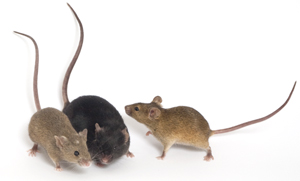
\includegraphics[width=0.8\linewidth]{009376}
%\captionof{figure}{\color{Green} DO mice demonstrate variation in body weight and fur color.}
%\end{center}\vspace{1cm}

\begin{center}\vspace{1cm}
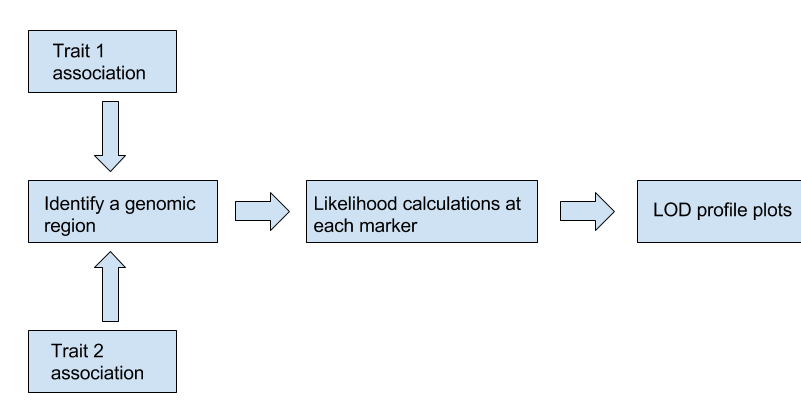
\includegraphics[width=\linewidth]{lrt-flow}
\captionof{figure}{\color{Green} Flow chart for our LRT procedure.}
\end{center}\vspace{1cm}




\subsection*{Evaluating the LRT with simulated data}

\begin{itemize}
\item Simulated multiple phenotypes with DO mouse estimated haplotype probabilities
\begin{itemize}
\item Varied inter-QTL distance when creating phenotypes
\end{itemize}
\item Assessed ability of LRT to distinguish pleiotropy from close linkage for distinct inter-QTL distances, $\lambda_1 - \lambda_2$.
\end{itemize}

\subsection*{Efforts to distinguish pleiotropy from close linkage in DO mouse phenotypes}

\begin{itemize}
\item Applied LRT to small genomic regions (~5 to 10 Mb) on chromosomes 3 and 17 to try to distinguish pleiotropy from close linkage
\end{itemize}

\begin{center}\vspace{1cm}
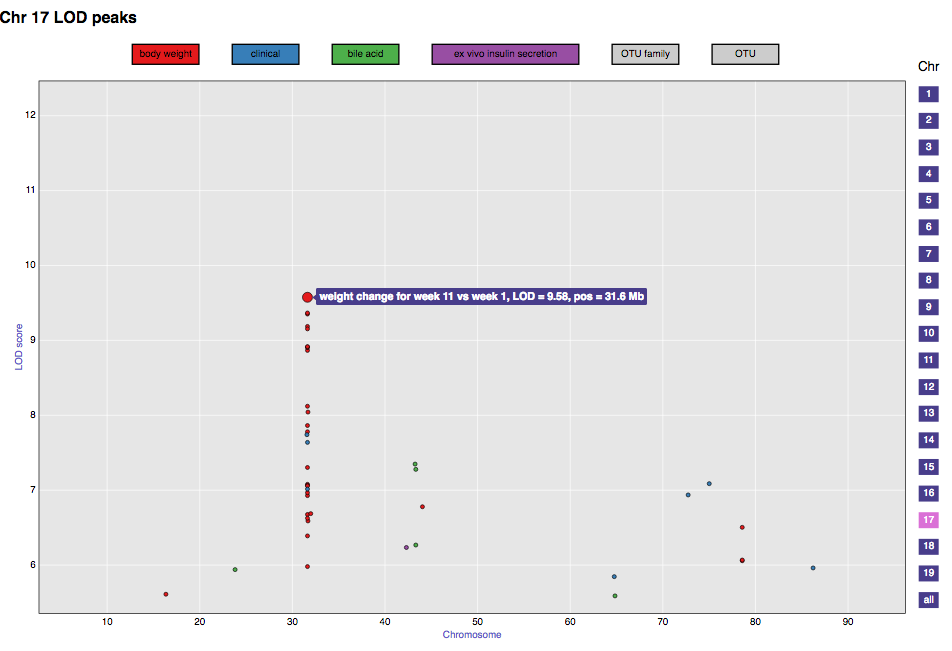
\includegraphics[width=0.8\linewidth]{lods-chr17}
\captionof{figure}{\color{Green} DO study LOD peaks on chromosome 17. Each point constitutes a LOD peak for one phenotype. Note that many phenotypes share a QTL near 31.6 Mb. Color corresponds to phenotype class, where red represents the class of body weight-related phenotypes, and purple is the class of insulin secretion phenotypes.}
\end{center}\vspace{1cm}



%----------------------------------------------------------------------------------------
%	RESULTS 
%----------------------------------------------------------------------------------------
\color{Navy}
\section*{Results}

\subsection*{Results with simulated phenotypes}

\begin{center}\vspace{1cm}
\includegraphics[width=0.8\linewidth]{unnamed-chunk-6-1.png}
\captionof{figure}{\color{Green} Close proximity of the two loci yields small profile LOD scores. We thus have little evidence against the null hypothesis of pleiotropy.}
\end{center}\vspace{1cm}

\begin{center}\vspace{1cm}
\includegraphics[width=0.8\linewidth]{unnamed-chunk-4-1.png}
\captionof{figure}{\color{Green} Profile LOD plots for two simulated traits with greater inter-locus distance.}
\end{center}\vspace{1cm}



\begin{itemize}
\item Used a normal linear model to simulate traits from loci in DO mice
\item Characterized our LRT by determining whether we could recover the true relationship (pleiotropy or close linkage) between the loci
\item For fixed effect sizes, greater inter-locus distances gave rise to higher LOD scores in our profile LOD plots.
\item \begin{equation}
\text{profile LOD}(\lambda_1) = \sup_{\lambda_2}LOD(\lambda_1, \lambda_2)
\end{equation}
\item \begin{equation}
\text{profile LOD}(\lambda_2) = \sup_{\lambda_1}LOD(\lambda_1, \lambda_2)
\end{equation}


\end{itemize}


\subsection*{Results with DO mice phenotypes}

\begin{itemize}
\item Chromosome 17 locus associates with multiple body weight phenotypes
\item Chromosome 3 locus associates with insulin secretion phenotypes
\end{itemize}


\begin{center}\vspace{1cm}
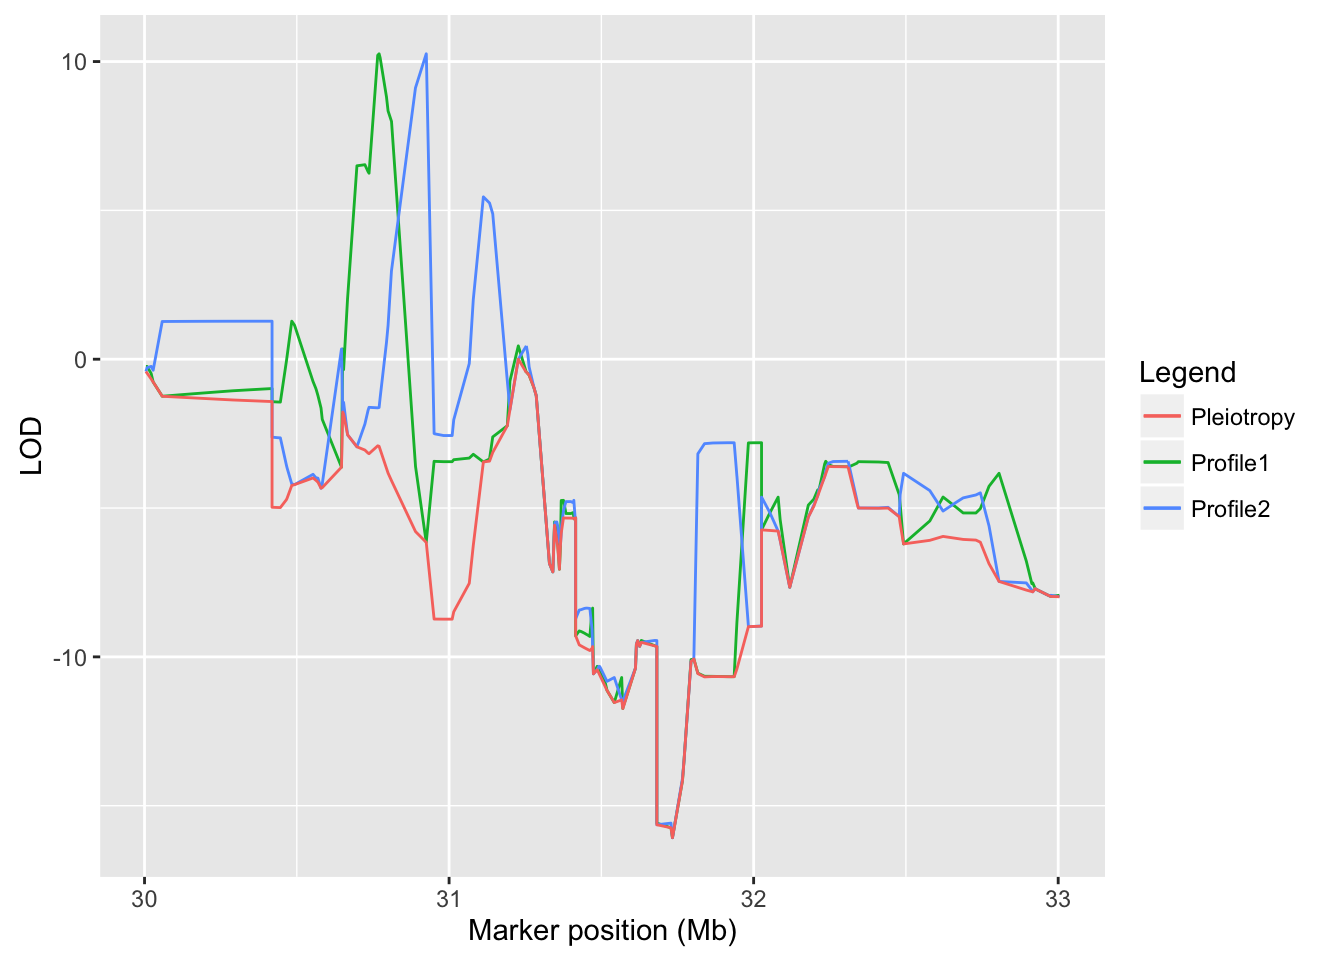
\includegraphics[width=0.8\linewidth]{do2.png}
\captionof{figure}{\color{Green} Weight change from week 1 to week 11 and weight change from week 1 to week 12 on chromosome 17}
\end{center}\vspace{1cm}

\begin{center}\vspace{1cm}
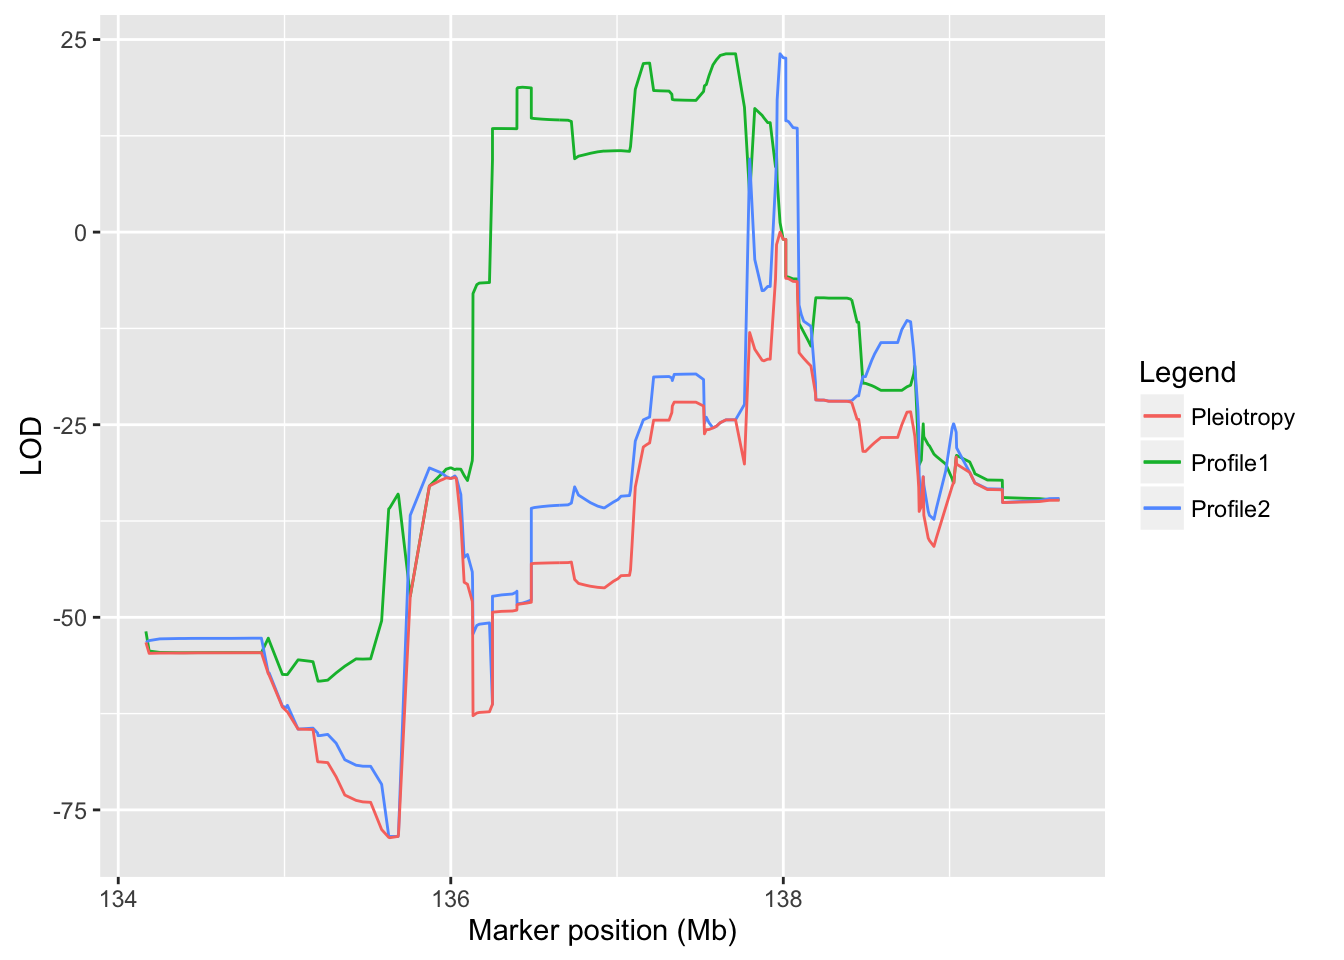
\includegraphics[width=0.8\linewidth]{do3.png}
\captionof{figure}{\color{Green} Chromosome 3 study with traits 1. Fraction of insulin secretion in response to amino acids and glucose and 2. Insulin secretion in response to GLP1 and glucose }
\end{center}\vspace{1cm}




\section*{Open Questions}

%%\begin{itemize}
%\item Simulation studies
%\begin{itemize}
%\item 
%\end{itemize}

%\item Investigations of chromosome 17 QTL
\begin{itemize}
\item Simulation studies suggest that we can distinguish pleiotropy from close linkage by examining the profile LOD plots
\item Our findings, in which we see low profile LOD scores, indicates little evidence against the null hypothesis of pleiotropy in both the chromosome 3 studies and the chromosome 17 studies
\item Future research will calibrate our LRT to distinguish pleiotropy from close linkage and will characterize its statistical power
\end{itemize}



%----------------------------------------------------------------------------------------
%	CONCLUSIONS
%----------------------------------------------------------------------------------------



\color{DarkSlateGray} % Set the color back to DarkSlateGray for the rest of the content

%----------------------------------------------------------------------------------------
%	FORTHCOMING RESEARCH
%----------------------------------------------------------------------------------------

%\section*{Forthcoming Research}



 %----------------------------------------------------------------------------------------
%	REFERENCES
%----------------------------------------------------------------------------------------


\bibliographystyle{plain} % Plain referencing style
\bibliography{sample} % Use the example bibliography file sample.bib

%----------------------------------------------------------------------------------------
%	ACKNOWLEDGEMENTS
%----------------------------------------------------------------------------------------

%\section*{Acknowledgements}

%Etiam fermentum, arcu ut gravida fringilla, dolor arcu laoreet justo, ut imperdiet urna arcu a arcu. Donec nec ante a dui tempus consectetur. Cras nisi turpis, dapibus sit amet mattis sed, laoreet.

%----------------------------------------------------------------------------------------

\end{multicols}
\end{document}